\documentclass[11pt,a4paper]{article}
\usepackage[margin=18mm,top=22mm,bottom=20mm]{geometry}
\usepackage{fontspec}\setmainfont{Latin Modern Roman}
\usepackage{xcolor}\usepackage{amsmath,amssymb,tikz,graphicx,fancyhdr,array,needspace}
\usetikzlibrary{patterns,arrows.meta,decorations.pathmorphing,calc}
\setlength{\headheight}{14pt}
\usetikzlibrary{arrows.meta}
\pagestyle{fancy}\fancyhf{}\renewcommand{\headrulewidth}{0.4pt}
\fancyhead[L]{\textbf{M-07}}\fancyhead[C]{\itshape Fizika — yechimlar (OliyFizika.uz)}\fancyhead[R]{\textbf{Mock №7}}
\fancyfoot[C]{\thepage}
\setlength{\parindent}{0pt}\setlength{\parskip}{3pt}
\newcommand{\opt}[2]{\hspace*{4mm}#1)\ #2\par}
\newcommand{\blank}{\rule{5cm}{0.4pt}}
\begin{document}

\begin{center}{\Large\textbf{FIZIKA — YECHIMLAR}}\\[2pt]{\large Mock №7}\end{center}
\Needspace{10\baselineskip}\noindent\begin{minipage}{\linewidth}
\textbf{1.}\ Tovuşni qaytarayotgan tösiqqaça masofa 68 m bölsa, qança vaqtdan (s) söng odam aks-sadoni eşitadi? Tovuş tezligi 340 m/s ga teng deb hisoblansin.\par\smallskip
\opt{A}{0,2}
\opt{B}{0,4}
\opt{C}{0,5}
\opt{D}{0,3}
\end{minipage}\vspace{2pt}\par
\noindent\colorbox{gray!12}{\parbox{\dimexpr\linewidth-2\fboxsep}{\textbf{Javob: B) 0,4}}}\par\smallskip
\noindent\textit{Yechim.}\ Tovuş tösiqqaça borib qaytadi: $t=\frac{2s}{v}=\frac{2\cdot68}{340}=0{,}4$ s.\par\par\medskip\hrule\medskip
\Needspace{10\baselineskip}\noindent\begin{minipage}{\linewidth}
\textbf{2.}\ Töğri çiziqli tekis tezlanuvçan harakat qilayotgan jismning $A$, $B$, $C$, $D$ nuqtalardagi kinetik energiyalari mos ravişda 0, $E$, $2E$, $3E$ ga teng. Agar $AB$ kesmaning uzunligi $S$ ga teng bölsa, $BC$ kesma uzunligini aniqlang.\par\smallskip
\opt{A}{$3S$}
\opt{B}{$3S/2$}
\opt{C}{$2S$}
\opt{D}{$S$}
\end{minipage}\vspace{2pt}\par
\noindent\colorbox{gray!12}{\parbox{\dimexpr\linewidth-2\fboxsep}{\textbf{Javob: D) $S$}}}\par\smallskip
\noindent\textit{Yechim.}\ Tinç holatdan tekis tezlanuvçan harakatda $E_k=Fs$, ya’ni kinetik energiya $A$ dan ötilgan yölga proporsional: $E$ ga $S$ yölda, $2E$ ga $2S$ yölda erişiladi. $BC=2S-S=S$.\par\par\medskip\hrule\medskip
\Needspace{10\baselineskip}\noindent\begin{minipage}{\linewidth}
\textbf{3.}\ Uzunligi 13 m va balandligi 5 m bölgan qiya tekislikda massasi 26 kg bölgan yuk yotibdi. Işqalaniş koeffitsiyenti 0,5 ga teng. Yukni yuqoriga çiqariş uçun tekislik böylab unga qanday kuç qöyiş lozim (N)? Tuşiriş uçunçi (N)? g=10 N/kg.\par\smallskip
\opt{A}{220; 20}
\opt{B}{200; 10}
\opt{C}{20; 10}
\opt{D}{5; 10}
\end{minipage}\vspace{2pt}\par
\noindent\colorbox{gray!12}{\parbox{\dimexpr\linewidth-2\fboxsep}{\textbf{Javob: A) 220; 20}}}\par\smallskip
\noindent\textit{Yechim.}\ $\sin\alpha=5/13$, $\cos\alpha=12/13$; $mg\sin\alpha=100$ N, $\mu mg\cos\alpha=0{,}5\cdot240=120$ N. Yuqoriga tekis çiqariş: $F_1=100+120=220$ N. Yuk özi sirpanmaydi ($100<120$); pastga tuşiriş uçun $F_2=120-100=20$ N.\par\par\medskip\hrule\medskip
\Needspace{10\baselineskip}\noindent\begin{minipage}{\linewidth}
\textbf{4.}\ Gorizontga nisbatan qiya örnatilgan diametri 1 cm bölgan quvurning uçidan yuqoriga qarab neft oqib çiqmoqda. Uning vertikal tezligi 30 m/s, gorizontal tezligi 1 m/s. 45 m balandlikda neft oqimining diametri (cm) qanday? g=10 m/s$^{2}$.\par\smallskip
\opt{A}{5,5}
\opt{B}{6}
\opt{C}{4,5}
\opt{D}{4}
\end{minipage}\vspace{2pt}\par
\noindent\colorbox{gray!12}{\parbox{\dimexpr\linewidth-2\fboxsep}{\textbf{Javob: A) 5,5}}}\par\smallskip
\noindent\textit{Yechim.}\ Oqim böylab $vS=\text{const}$. Quvur uçida $v_1=\sqrt{30^2+1^2}\approx30$ m/s. 45 m balandlikda vertikal tezlik $v_y^2=900-2\cdot10\cdot45=0$, ya’ni $v_2=1$ m/s.\par
\[\frac{d_2^2}{d_1^2}=\frac{v_1}{v_2}\approx30\ \Rightarrow\ d_2\approx1\cdot\sqrt{30}\approx5{,}5\ \text{cm}.\]\par\medskip\hrule\medskip
\Needspace{10\baselineskip}\noindent\begin{minipage}{\linewidth}
\textbf{5.}\ Öqning massasi 10 g. Öq havoda tovuş tezligida (330 m/s) uçişi uçun miltiqda unga qanday doimiy kuç (N) ta’sir etişi kerak? Öqning miltiqdan uçib çiqiş davomiyligi 0,001 s.\par\smallskip
\opt{A}{4400}
\opt{B}{6600}
\opt{C}{2200}
\opt{D}{3300}
\end{minipage}\vspace{2pt}\par
\noindent\colorbox{gray!12}{\parbox{\dimexpr\linewidth-2\fboxsep}{\textbf{Javob: D) 3300}}}\par\smallskip
\noindent\textit{Yechim.}\ $Ft=mv$: $F=\frac{0{,}01\cdot330}{0{,}001}=3300$ N.\par\par\medskip\hrule\medskip
\Needspace{10\baselineskip}\noindent\begin{minipage}{\linewidth}
\textbf{6.}\ Darsga kelayotgan öquvçi oldin yölning 3 km ni 20 min da bosib ötdi va yölda uxlab qoldi. Uyğongaç qolgan 3 km yölni yana 20 min da bosib ötib, darsga keçikib keldi. Agar öquvçining butun yöldagi örtaça tezligi 3 km/h bölsa, u yölda neça minut uxlab qolgan?\par\smallskip
\opt{A}{90}
\opt{B}{70}
\opt{C}{80}
\opt{D}{60}
\end{minipage}\vspace{2pt}\par
\noindent\colorbox{gray!12}{\parbox{\dimexpr\linewidth-2\fboxsep}{\textbf{Javob: C) 80}}}\par\smallskip
\noindent\textit{Yechim.}\ Butun yöl 6 km, örtaça tezlik 3 km/h — umumiy vaqt 2 soat $=120$ min. Yurişga $20+20=40$ min ketgan, uxlagan vaqt $120-40=80$ min.\par\par\medskip\hrule\medskip
\Needspace{10\baselineskip}\noindent\begin{minipage}{\linewidth}
\textbf{7.}\ Kosmik vaznsizlikda muallaq turgan aylana kosmik stansiyada sun’iy gravitatsiya hosil qiliş uçun uning dvigatellari işga tuşib stansiya öz öqi atrofida bir tekisda aylana boşladi. Stansiya radiusi 40 m bölsa, stansiyada yerdagidek gravitasiya yuzaga kelişi uçun u öz öqi atrofida qanday burçak tezlikda aylanişi kerak (rad/s)? Yerda erkin tuşiş tezlanişi 10 N/kg.\par\smallskip
\opt{A}{1}
\opt{B}{2}
\opt{C}{0,5}
\opt{D}{0,2}
\end{minipage}\vspace{2pt}\par
\noindent\colorbox{gray!12}{\parbox{\dimexpr\linewidth-2\fboxsep}{\textbf{Javob: C) 0,5}}}\par\smallskip
\noindent\textit{Yechim.}\ Stansiya devori odamga markazga intilma tezlaniş beradi: $\omega^2R=g$, $\omega=\sqrt{10/40}=0{,}5$ rad/s.\par\par\medskip\hrule\medskip
\Needspace{10\baselineskip}\noindent\begin{minipage}{\linewidth}
\textbf{8.}\ Jismning turğunligi (barqarorligi) yuqori böliş sifatlarini körsating. 1) jism oğirligining kattaligi; 2) jism asosi yuzining kattaligi; 3) jism oğirligining kiçikligi; 4) jism asosi yuzining kiçikligi.\par\smallskip
\opt{A}{1,2,}
\opt{B}{2,3, 4}
\opt{C}{1,3,4}
\opt{D}{1,3}
\end{minipage}\vspace{2pt}\par
\noindent\colorbox{gray!12}{\parbox{\dimexpr\linewidth-2\fboxsep}{\textbf{Javob: A) 1,2,}}}\par\smallskip
\noindent\textit{Yechim.}\ Jism oğirligi qança katta va tayanç yuzasi qança keng bölsa, uni ağdariş şunça qiyin: 1 va 2.\par\par\medskip\hrule\medskip
\Needspace{10\baselineskip}\noindent\begin{minipage}{\linewidth}
\textbf{9.}\ Töğri çiziqli tekis sekinlanuvçan harakat qilayotgan jism beşinçi sekundda 5 m yöl bosdi va töxtadi. Harakatning ikkinçi sekundida jism qanday yöl (m) bosib ötadi?\par\smallskip
\opt{A}{35}
\opt{B}{14}
\opt{C}{25}
\opt{D}{75}
\end{minipage}\vspace{2pt}\par
\noindent\colorbox{gray!12}{\parbox{\dimexpr\linewidth-2\fboxsep}{\textbf{Javob: A) 35}}}\par\smallskip
\noindent\textit{Yechim.}\ Oxirgi (5-) sekundda $s=\frac{a\cdot1^2}{2}=5$, $a=10$ m/s$^2$; $v_0=at=50$ m/s. Ikkinçi sekunddagi yöl\par
\[s_2=v_0-a\left(2-\frac12\right)=50-15=35\ \text{m}.\]\par\medskip\hrule\medskip
\Needspace{10\baselineskip}\noindent\begin{minipage}{\linewidth}
\textbf{10.}\ Ikki sterjen berilgan, mos ravişda ularning uzunliklari $l_1$ va $l_2$, çiziqli ziçliklari $\rho_1$ va $\rho_2$. Sterjenlarni rasmda körsatilganidek birlaştirsak, hosil bölgan sterjenda oğirlik kuçlari birinçi sterjenning taşqi uçiga nisbatan qanday kuç momenti hosil qiladi?\par\smallskip
\noindent\hspace*{4mm}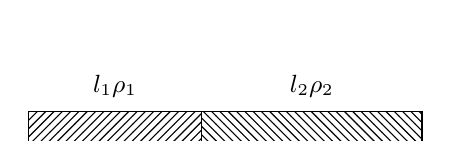
\begin{tikzpicture}[x=1cm,y=1cm,line width=0.5pt,>=Stealth,font=\small]
\draw[pattern=north east lines] (0,0) rectangle (2.2,0.5); \draw[pattern=north west lines] (2.2,0) rectangle (5,0.5);
\node[above] at (1.1,0.55) {$l_1\rho_1$}; \node[above] at (3.6,0.55) {$l_2\rho_2$};
\end{tikzpicture}\par\smallskip
\opt{A}{$\dfrac{g}{2}(\rho_1l_1^2+\rho_2l_2^2+2\rho_2l_1l_2)$}
\opt{B}{$g(\rho_1l_1^2+\rho_2l_2^2+2\rho_2l_1l_2)$}
\opt{C}{$\dfrac{g}{2}(l_1^2\rho_1+l_2^2\rho_2+l_1l_2\rho_2)$}
\opt{D}{$\dfrac{g}{2}(l_1^2\rho_1+l_2^3\rho_2+2l_1l_2\rho_2)$}
\end{minipage}\vspace{2pt}\par
\noindent\colorbox{gray!12}{\parbox{\dimexpr\linewidth-2\fboxsep}{\textbf{Javob: A) $\dfrac{g}{2}(\rho_1l_1^2+\rho_2l_2^2+2\rho_2l_1l_2)$}}}\par\smallskip
\noindent\textit{Yechim.}\ Birinçi sterjen oğirlik markazi taşqi uçdan $l_1/2$, ikkinçisiniki $l_1+l_2/2$ masofada:\par
\[M=\rho_1l_1g\frac{l_1}{2}+\rho_2l_2g\left(l_1+\frac{l_2}{2}\right)=\frac{g}{2}\left(\rho_1l_1^2+\rho_2l_2^2+2\rho_2l_1l_2\right).\]\par\medskip\hrule\medskip
\Needspace{10\baselineskip}\noindent\begin{minipage}{\linewidth}
\textbf{11.}\ Qaynab turgan suyuqlikka taşqaridan issiqlik miqdori berişda davom etsak uning temperaturasi qanday özgaradi?\par\smallskip
\opt{A}{avval kamayib keyin ortadi}
\opt{B}{kamayadi}
\opt{C}{özgarmaydi}
\opt{D}{ortadi}
\end{minipage}\vspace{2pt}\par
\noindent\colorbox{gray!12}{\parbox{\dimexpr\linewidth-2\fboxsep}{\textbf{Javob: C) özgarmaydi}}}\par\smallskip
\noindent\textit{Yechim.}\ Qaynaş davomida berilgan issiqlik buğlanişga sarflanadi, temperatura özgarmaydi.\par\par\medskip\hrule\medskip
\Needspace{10\baselineskip}\noindent\begin{minipage}{\linewidth}
\textbf{12.}\ Vertikal joylaştirilgan uzun silindrik germetik idiş porşen orqali ikkiga ajratilgan. Porşen ostida 2 mol, yuqorisida esa 3 mol havo bor. Idişdagi temperatura 300 K bölgan paytda silindr yuqorisidagi gaz hajmi pastdagi gaz hajmidan 3 marta katta böldi. Qanday temperaturada (K) gaz hajmlari 4 marta farq qiladi?\par\smallskip
\opt{A}{112}
\opt{B}{144}
\opt{C}{156}
\opt{D}{192}
\end{minipage}\vspace{2pt}\par
\noindent\colorbox{gray!12}{\parbox{\dimexpr\linewidth-2\fboxsep}{\textbf{Javob: D) 192}}}\par\smallskip
\noindent\textit{Yechim.}\ Porşen oğirligi tufayli pastki bosim $p_1=p_2+\Delta p$, $\Delta p$ özgarmas. Idiş hajmi $V$. 300 K da: $V_1=V/4$, $V_2=3V/4$, $p_1=\frac{8RT}{V}$, $p_2=\frac{4RT}{V}$, $\Delta p=\frac{4R\cdot300}{V}$. $T$ da: $V_1=V/5$, $V_2=4V/5$, $p_1=\frac{10RT}{V}$, $p_2=\frac{3{,}75RT}{V}$, $\Delta p=\frac{6{,}25RT}{V}$.\par
\[6{,}25T=1200\ \Rightarrow\ T=192\ \text{K}.\]\par\medskip\hrule\medskip
\Needspace{10\baselineskip}\noindent\begin{minipage}{\linewidth}
\textbf{13.}\ Nisbiy molekular massasi $M_r = 32$ u ga teng bölgan moddaning massasini (g) aniqlang. 1 u=$1{,}66\cdot10^{-27}$ kg\par\smallskip
\opt{A}{$53{,}12\cdot10^{-30}$}
\opt{B}{$5{,}312\cdot10^{-27}$}
\opt{C}{$53{,}12\cdot10^{-24}$}
\opt{D}{$53{,}12\cdot10^{-27}$}
\end{minipage}\vspace{2pt}\par
\noindent\colorbox{gray!12}{\parbox{\dimexpr\linewidth-2\fboxsep}{\textbf{Javob: C) $53{,}12\cdot10^{-24}$}}}\par\smallskip
\noindent\textit{Yechim.}\ $m=32\cdot1{,}66\cdot10^{-27}$ kg $=5{,}312\cdot10^{-26}$ kg $=53{,}12\cdot10^{-24}$ g.\par\par\medskip\hrule\medskip
\Needspace{10\baselineskip}\noindent\begin{minipage}{\linewidth}
\textbf{14.}\ 177 $^\circ$C temperaturali 12 g gaz 4 l hajmga ega. Bosim özgarmas bölsa, gaz ziçligi qanday temperaturada 6 kg/m$^{3}$ ga teng böladi (K)?\par\smallskip
\opt{A}{225}
\opt{B}{255}
\opt{C}{260}
\opt{D}{275}
\end{minipage}\vspace{2pt}\par
\noindent\colorbox{gray!12}{\parbox{\dimexpr\linewidth-2\fboxsep}{\textbf{Javob: A) 225}}}\par\smallskip
\noindent\textit{Yechim.}\ Dastlabki ziçlik $\rho_1=12/4=3$ kg/m$^3$ ($T_1=450$ K). Izobarik jarayonda $\rho T=\text{const}$:\par
\[T_2=T_1\frac{\rho_1}{\rho_2}=450\cdot\frac36=225\ \text{K}.\]\par\medskip\hrule\medskip
\Needspace{10\baselineskip}\noindent\begin{minipage}{\linewidth}
\textbf{15.}\ Kislorod gaziga berilgan issiqlik miqdorining yarmi taşqi kuçlarga qarşi iş bajarişga sarflandi. Agar bu jarayonda gazning içki energiyasi 120 J ga ortgan bölsa, gazga berilgan issiqlik miqdorini (J) aniqlang.\par\smallskip
\opt{A}{240}
\opt{B}{200}
\opt{C}{120}
\opt{D}{168}
\end{minipage}\vspace{2pt}\par
\noindent\colorbox{gray!12}{\parbox{\dimexpr\linewidth-2\fboxsep}{\textbf{Javob: A) 240}}}\par\smallskip
\noindent\textit{Yechim.}\ $Q=\Delta U+A$, $A=Q/2$, demak $\Delta U=Q/2=120$ J, $Q=240$ J.\par\par\medskip\hrule\medskip
\Needspace{10\baselineskip}\noindent\begin{minipage}{\linewidth}
\textbf{16.}\ Zaryadlangan şarning sirtiy ziçligi 4 nC/m$^{2}$, radiusi 8,85 cm bölsa, şarning sirtidan uning radiusiga teng masofadagi maydon potensialini toping (V). $\varepsilon$=2.\par\smallskip
\opt{A}{5}
\opt{B}{20}
\opt{C}{15}
\opt{D}{10}
\end{minipage}\vspace{2pt}\par
\noindent\colorbox{gray!12}{\parbox{\dimexpr\linewidth-2\fboxsep}{\textbf{Javob: D) 10}}}\par\smallskip
\noindent\textit{Yechim.}\ $q=\sigma\cdot4\pi R^2$. Sirtdan $R$ masofada ($r=2R$):\par
\[\varphi=\frac{q}{4\pi\varepsilon_0\varepsilon\cdot2R}=\frac{\sigma R}{2\varepsilon_0\varepsilon}=\frac{4\cdot10^{-9}\cdot0{,}0885}{2\cdot8{,}85\cdot10^{-12}\cdot2}=10\ \text{V}.\]\par\medskip\hrule\medskip
\Needspace{10\baselineskip}\noindent\begin{minipage}{\linewidth}
\textbf{17.}\ Doimiy tok manbai içidagi çet kuçlar 6 C zaryadni elektrostatik kuçlarga qarşi yönalişda köçirişda 300 J iş bajardi. Tok manbaining EYK ini toping (V).\par\smallskip
\opt{A}{0,02}
\opt{B}{25}
\opt{C}{50}
\opt{D}{450}
\end{minipage}\vspace{2pt}\par
\noindent\colorbox{gray!12}{\parbox{\dimexpr\linewidth-2\fboxsep}{\textbf{Javob: C) 50}}}\par\smallskip
\noindent\textit{Yechim.}\ $\mathcal E=A_{ch}/q=300/6=50$ V.\par\par\medskip\hrule\medskip
\Needspace{10\baselineskip}\noindent\begin{minipage}{\linewidth}
\textbf{18.}\ Qarşiligi 0,9 $\Omega$ bölgan ampermetrning ölçaş çegarasini 10 marta orttiriş uçun unga qanday qarşilikli şunt ulaş kerak ($\Omega$)?\par\smallskip
\opt{A}{0,01}
\opt{B}{0,1}
\opt{C}{0,3}
\opt{D}{1}
\end{minipage}\vspace{2pt}\par
\noindent\colorbox{gray!12}{\parbox{\dimexpr\linewidth-2\fboxsep}{\textbf{Javob: B) 0,1}}}\par\smallskip
\noindent\textit{Yechim.}\ $R_{sh}=\frac{R_A}{n-1}=\frac{0{,}9}{9}=0{,}1\ \Omega$.\par\par\medskip\hrule\medskip
\Needspace{10\baselineskip}\noindent\begin{minipage}{\linewidth}
\textbf{19.}\ Qarşiligi 1 $\Omega$ bölgan silindrsimon ötkazgiç uçlariga 16 V kuçlaniş qöyilgan. Bu ötkazgiçning köndalang kesimidan 5 s da neçta elektron ötadi? $e = 1{,}6\cdot10^{-19}$ C\par\smallskip
\opt{A}{$50\cdot10^{19}$}
\opt{B}{$500\cdot10^{19}$}
\opt{C}{$50\cdot10^{17}$}
\opt{D}{$5\cdot10^{19}$}
\end{minipage}\vspace{2pt}\par
\noindent\colorbox{gray!12}{\parbox{\dimexpr\linewidth-2\fboxsep}{\textbf{Javob: A) $50\cdot10^{19}$}}}\par\smallskip
\noindent\textit{Yechim.}\ $I=U/R=16$ A, $q=It=80$ C, $N=\frac{q}{e}=\frac{80}{1{,}6\cdot10^{-19}}=5\cdot10^{20}=50\cdot10^{19}$.\par\par\medskip\hrule\medskip
\Needspace{10\baselineskip}\noindent\begin{minipage}{\linewidth}
\textbf{20.}\ Fazodagi $A$ nuqtada elektromagnit tölqin $y$ öqi böylab tarqalmoqda. Uning elektr maydon kuçlanganligi $x$ koordinata öqi böylab yönalgan. Tölqinning magnit maydon induksiyasi qanday yönalgan?\par\smallskip
\opt{A}{$z$ öqiga qarşi}
\opt{B}{$z$ öqi böylab}
\opt{C}{$y$ öqiga qarşi}
\opt{D}{$y$ öqi böylab}
\end{minipage}\vspace{2pt}\par
\noindent\colorbox{gray!12}{\parbox{\dimexpr\linewidth-2\fboxsep}{\textbf{Javob: A) $z$ öqiga qarşi}}}\par\smallskip
\noindent\textit{Yechim.}\ Elektromagnit tölqinda $\vec E$, $\vec B$ va tarqaliş yönalişi öng vint sistemasini taşkil qiladi: $[\vec E\times\vec B]$ tarqaliş tomonga. $[\hat x\times(-\hat z)]=\hat y$, demak $\vec B$ $z$ öqiga qarşi.\par\par\medskip\hrule\medskip
\Needspace{10\baselineskip}\noindent\begin{minipage}{\linewidth}
\textbf{21.}\ 100 cm$^{2}$ sirtga har minutda 60 J elektromagnit tölqin energiyasi kelib tuşmoqda. Elektromagnit tölqinning intensivligini toping (W/m$^{2}$).\par\smallskip
\opt{A}{110}
\opt{B}{100}
\opt{C}{120}
\opt{D}{150}
\end{minipage}\vspace{2pt}\par
\noindent\colorbox{gray!12}{\parbox{\dimexpr\linewidth-2\fboxsep}{\textbf{Javob: B) 100}}}\par\smallskip
\noindent\textit{Yechim.}\ \[I=\frac{W}{St}=\frac{60}{0{,}01\cdot60}=100\ \text{W/m}^2.\]\par\medskip\hrule\medskip
\Needspace{10\baselineskip}\noindent\begin{minipage}{\linewidth}
\textbf{22.}\ Tomoni $a$ bölgan teng tomonli uçburçakning uçlarida $q$, $2q$, $3q$ zaryadli nuqtaviy zarralar joylaşgan. Zaryadi $2q$, massasi $m$ bölgan zarra böşatib yuborilsa, u qanday maksimal tezlikka erişadi?\par\smallskip
\opt{A}{$\sqrt{\dfrac{18kq^2}{ma}}$}
\opt{B}{$\sqrt{\dfrac{6kq}{ma}}$}
\opt{C}{$\sqrt{\dfrac{18kq}{ma}}$}
\opt{D}{$\sqrt{\dfrac{16kq^2}{ma}}$}
\end{minipage}\vspace{2pt}\par
\noindent\colorbox{gray!12}{\parbox{\dimexpr\linewidth-2\fboxsep}{\textbf{Javob: D) $\sqrt{\dfrac{16kq^2}{ma}}$}}}\par\smallskip
\noindent\textit{Yechim.}\ $2q$ zaryadning qolgan zaryadlar bilan ta’sir energiyasi $W=\frac{k\cdot2q(q+3q)}{a}=\frac{8kq^2}{a}$ — u töliq kinetik energiyaga aylanadi:\par
\[\frac{mv^2}{2}=\frac{8kq^2}{a}\ \Rightarrow\ v=\sqrt{\frac{16kq^2}{ma}}.\]\par\medskip\hrule\medskip
\Needspace{10\baselineskip}\noindent\begin{minipage}{\linewidth}
\textbf{23.}\ Agar ğaltak 100 ta öramga ega bölganda, unda 120 V EyuK hosil bölsa, uning içida magnit oqimi 0,05 s davomida qançaga (mWb) özgaradi?\par\smallskip
\opt{A}{90}
\opt{B}{30}
\opt{C}{60}
\opt{D}{80}
\end{minipage}\vspace{2pt}\par
\noindent\colorbox{gray!12}{\parbox{\dimexpr\linewidth-2\fboxsep}{\textbf{Javob: C) 60}}}\par\smallskip
\noindent\textit{Yechim.}\ $\mathcal E=N\frac{\Delta\Phi}{\Delta t}$: $\Delta\Phi=\frac{120\cdot0{,}05}{100}=0{,}06$ Wb $=60$ mWb.\par\par\medskip\hrule\medskip
\Needspace{10\baselineskip}\noindent\begin{minipage}{\linewidth}
\textbf{24.}\ Qarşiligi 10 $\Omega$ bölgan rezistorga qarşiligi 15 $\Omega$ bölgan rezistor parallel ulandi. Zanjirning umumiy qarşiligi 10 $\Omega$ bölişi uçun bu ikki rezistorga ketma-ket qilib qanday qarşilikni ulaş kerak ($\Omega$)?\par\smallskip
\opt{A}{3}
\opt{B}{2}
\opt{C}{1}
\opt{D}{4}
\end{minipage}\vspace{2pt}\par
\noindent\colorbox{gray!12}{\parbox{\dimexpr\linewidth-2\fboxsep}{\textbf{Javob: D) 4}}}\par\smallskip
\noindent\textit{Yechim.}\ $R_{par}=\frac{10\cdot15}{25}=6\ \Omega$; ketma-ket $10-6=4\ \Omega$ ulaş kerak.\par\par\medskip\hrule\medskip
\Needspace{10\baselineskip}\noindent\begin{minipage}{\linewidth}
\textbf{25.}\ E.Yu.K $\varepsilon$ bölgan tok manbaida qisqa tutaşuv yuz berdi. Mazkur holatda manba qutblaridagi $U$ kuçlanişni toping.\par\smallskip
\opt{A}{$U=\varepsilon$}
\opt{B}{0}
\opt{C}{$U<\varepsilon$}
\opt{D}{$U>\varepsilon$}
\end{minipage}\vspace{2pt}\par
\noindent\colorbox{gray!12}{\parbox{\dimexpr\linewidth-2\fboxsep}{\textbf{Javob: B) 0}}}\par\smallskip
\noindent\textit{Yechim.}\ Qisqa tutaşuvda taşqi qarşilik nol: $U=IR=0$ (butun EYuK içki qarşilikka tuşadi).\par\par\medskip\hrule\medskip
\Needspace{10\baselineskip}\noindent\begin{minipage}{\linewidth}
\textbf{26.}\ Optik kuçi 2 D bölgan yiğuvçi linzadan ikkilangan fokus masofada turgan buyum 1 m/s tezlik bilan linza tomon harakatlana boşladi. Bundan 0,75 s vaqt ötgan paytda buyum va uning tasviri orasidagi masofa qanday böladi (m)?\par\smallskip
\opt{A}{0,5}
\opt{B}{0,25}
\opt{C}{0,75}
\opt{D}{0,15}
\end{minipage}\vspace{2pt}\par
\noindent\colorbox{gray!12}{\parbox{\dimexpr\linewidth-2\fboxsep}{\textbf{Javob: B) 0,25}}}\par\smallskip
\noindent\textit{Yechim.}\ $F=0{,}5$ m, buyum dastlab $2F=1$ m da. 0,75 s da $0{,}75$ m yaqinlaşadi: $d=0{,}25$ m $<F$, tasvir mavhum:\par
\[\frac1f=\frac1F-\frac1d=2-4=-2\ \Rightarrow\ |f|=0{,}5\ \text{m}\ \text{(buyum tomonda)}.\]
Buyum va tasvir orasidagi masofa $0{,}5-0{,}25=0{,}25$ m.\par\par\medskip\hrule\medskip
\Needspace{10\baselineskip}\noindent\begin{minipage}{\linewidth}
\textbf{27.}\ Linzaning fokal tekisligi deb nimaga aytiladi?\par\smallskip
\opt{A}{linza markazidan ötgan tekislik}
\opt{B}{boş optik öqqa parallel tekislik}
\opt{C}{boş optik öqqa 45$^\circ$ burçak ostida ötgan tekislik}
\opt{D}{linza fokuslaridan boş optik öqqa perpendikulyar ötgan tekisliklar}
\end{minipage}\vspace{2pt}\par
\noindent\colorbox{gray!12}{\parbox{\dimexpr\linewidth-2\fboxsep}{\textbf{Javob: D) linza fokuslaridan boş optik öqqa perpendikulyar ötgan tekisliklar}}}\par\smallskip
\noindent\textit{Yechim.}\ Fokal tekislik — linza fokusidan boş optik öqqa perpendikulyar ötgan tekislik.\par\par\medskip\hrule\medskip
\Needspace{10\baselineskip}\noindent\begin{minipage}{\linewidth}
\textbf{28.}\ Elektr yoritgiç radiusi 10 cm, yoruğlik kuçi 100 cd bölgan şardan iborat. Manbaning töla yoruğlik oqimini toping (lm).\par\smallskip
\opt{A}{1256}
\opt{B}{1500}
\opt{C}{1700}
\opt{D}{1800}
\end{minipage}\vspace{2pt}\par
\noindent\colorbox{gray!12}{\parbox{\dimexpr\linewidth-2\fboxsep}{\textbf{Javob: A) 1256}}}\par\smallskip
\noindent\textit{Yechim.}\ Nuqtaviy (izotrop) manba uçun $\Phi=4\pi I=4\cdot3{,}14\cdot100=1256$ lm.\par\par\medskip\hrule\medskip
\Needspace{10\baselineskip}\noindent\begin{minipage}{\linewidth}
\textbf{29.}\ Vodorod atomidagi 1-energetik sathda bölgan elektronning kinetik energiyasi (eV) qanday? Asosiy holatdagi vodorod atomini ionlaştiriş energiyasi 13,6 eV.\par\smallskip
\opt{A}{10,2}
\opt{B}{13,6}
\opt{C}{3,4}
\opt{D}{6,8}
\end{minipage}\vspace{2pt}\par
\noindent\colorbox{gray!12}{\parbox{\dimexpr\linewidth-2\fboxsep}{\textbf{Javob: B) 13,6}}}\par\smallskip
\noindent\textit{Yechim.}\ Bor modelida elektronning kinetik energiyasi töliq energiyaning moduliga teng: $E_k=|E_1|=13{,}6$ eV.\par\par\medskip\hrule\medskip
\Needspace{10\baselineskip}\noindent\begin{minipage}{\linewidth}
\textbf{30.}\ Zarrada 2 ta elektron, 3 ta neytron va 4 ta proton bölsa, uşbu zarrani toping.\par\smallskip
\opt{A}{$^{7}_{3}$Li atomi}
\opt{B}{$^{7}_{4}$Be ioni}
\opt{C}{$^{7}_{4}$Be atomi}
\opt{D}{$^{9}_{4}$Be atomi}
\end{minipage}\vspace{2pt}\par
\noindent\colorbox{gray!12}{\parbox{\dimexpr\linewidth-2\fboxsep}{\textbf{Javob: B) $^{7}_{4}$Be ioni}}}\par\smallskip
\noindent\textit{Yechim.}\ 4 ta proton — berilliy ($Z=4$), massa soni $A=4+3=7$. Elektronlar 2 ta, ya’ni 2 ta elektron yetişmaydi — bu $^7_4$Be ioni ($Be^{2+}$).\par\par\medskip\hrule\medskip
\Needspace{10\baselineskip}\noindent\begin{minipage}{\linewidth}
\textbf{31.}\ Ketma-ket keladigan ikkita $\alpha$-yemirilişdan söng yadrodagi protonlar soni....\par\smallskip
\opt{A}{ikkitaga kamayadi}
\opt{B}{uçtaga kamayadi}
\opt{C}{özgarmaydi}
\opt{D}{törttaga kamayadi}
\end{minipage}\vspace{2pt}\par
\noindent\colorbox{gray!12}{\parbox{\dimexpr\linewidth-2\fboxsep}{\textbf{Javob: D) törttaga kamayadi}}}\par\smallskip
\noindent\textit{Yechim.}\ Har bir $\alpha$-yemirilişda yadro zaryadi 2 ga kamayadi; ikkitasidan söng protonlar soni 4 taga kamayadi.\par\par\medskip\hrule\medskip
\Needspace{10\baselineskip}\noindent\begin{minipage}{\linewidth}
\textbf{32.}\ Jism tezligi v = 12 $-$ 2t [m/s] qonuniyat bilan özgarmoqda. Uning 3 s dan keyingi oniy tezligi qança (m/s) böladi?\par\smallskip
\opt{A}{2}
\opt{B}{6}
\opt{C}{4}
\opt{D}{8}
\end{minipage}\vspace{2pt}\par
\noindent\colorbox{gray!12}{\parbox{\dimexpr\linewidth-2\fboxsep}{\textbf{Javob: B) 6}}}\par\smallskip
\noindent\textit{Yechim.}\ $v(3)=12-2\cdot3=6$ m/s.\par\par\medskip\hrule\medskip
\newpage\noindent\textbf{33–35.}\ Rasmdagi zanjirda $\varepsilon=12$ V, $r=1\ \Omega$, $R_1=3\ \Omega$, $R_2=2\ \Omega$, $C=5\ \mu$F. Zanjirda tok qaror topgan.\par\medskip
\begin{center}\begin{tikzpicture}[x=1cm,y=1cm,line width=0.5pt,>=Stealth,font=\small]
\draw (0,0)--(0,0.6) (0,0.9)--(0,1.8)--(1.2,1.8); \draw (-0.3,0.9)--(0.3,0.9) (-0.15,0.6)--(0.15,0.6); \node[left] at (-0.35,0.75) {$\varepsilon, r$};
\draw[fill=white] (1.2,1.65) rectangle (2.0,1.95); \node[above] at (1.6,1.95) {$R_1$}; \draw (2.0,1.8)--(3.0,1.8)--(3.0,1.3) (3.0,0.5)--(3.0,0)--(0,0);
\draw[fill=white] (2.85,0.5) rectangle (3.15,1.3); \node[left] at (2.8,0.9) {$R_2$};
\draw (3.0,1.8)--(4.2,1.8)--(4.2,1.05) (4.2,0.75)--(4.2,0)--(3.0,0); \draw (3.9,1.05)--(4.5,1.05) (3.9,0.75)--(4.5,0.75); \node[right] at (4.5,0.9) {$C$};
\fill (3.0,1.8) circle(1.2pt) (3.0,0) circle(1.2pt);
\end{tikzpicture}\end{center}
\noindent\textbf{33.}\ Manbadan ötayotgan tok kuçini (A) toping.\par
\noindent\textbf{34.}\ Kondensatordagi kuçlanişni (V) toping.\par
\noindent\textbf{35.}\ Kondensatordagi zaryadni ($\mu$C) toping.\par
\noindent Variantlar: A) 2;\quad B) 2,4;\quad C) 4;\quad D) 6;\quad E) 20;\quad F) 30\par\smallskip
\noindent\colorbox{gray!12}{\parbox{\dimexpr\linewidth-2\fboxsep}{\textbf{Javob: 33--A) 2; 34--C) 4; 35--E) 20}}}\par\smallskip
\noindent\textit{Yechim.}\ Qaror topgan rejimda kondensator orqali tok ötmaydi: $I=\frac{\varepsilon}{R_1+R_2+r}=\frac{12}{6}=2$ A. Kondensator $R_2$ ga parallel: $U_C=IR_2=4$ V, $q=CU_C=5\cdot4=20\ \mu$C.\par\par\medskip\hrule\medskip
\Needspace{12\baselineskip}\noindent\textbf{36.}\ Hajmi 2 dm$^3$, massasi 0,5 kg bölgan şar idiş tubiga boğlangan ip yordamida suv içida töliq botgan holda uşlab turilibdi. $\rho_{suv}=1000$ kg/m$^3$, $g=10$ m/s$^2$.\par
\noindent\hspace*{4mm}a)\ Şarga ta’sir qiluvçi Arximed kuçini (N) toping.\par
\noindent\hspace*{4mm}b)\ Ipning taranglik kuçini (N) toping.\par
\noindent\colorbox{gray!12}{\parbox{\dimexpr\linewidth-2\fboxsep}{\textbf{Javob: a)\ 20;\quad b)\ 15}}}\par\smallskip
\noindent\textit{Yechim.}\ $F_A=\rho_s gV=1000\cdot10\cdot2\cdot10^{-3}=20$ N. Muvozanat: $F_A=mg+T$, $T=20-5=15$ N.\par\par\medskip\hrule\medskip
\Needspace{12\baselineskip}\noindent\textbf{37.}\ Kengligi 120 m bölgan daryoni qayiq oqimga tik yönalişda suvga nisbatan 4 m/s tezlik bilan suzib kesib ötmoqda. Daryo oqimining tezligi 3 m/s.\par
\noindent\hspace*{4mm}a)\ Qayiqning daryoni kesib ötiş vaqtini (s) toping.\par
\noindent\hspace*{4mm}b)\ Qayiq oqim böylab qança masofaga (m) surilib ketadi?\par
\noindent\colorbox{gray!12}{\parbox{\dimexpr\linewidth-2\fboxsep}{\textbf{Javob: a)\ 30;\quad b)\ 90}}}\par\smallskip
\noindent\textit{Yechim.}\ $t=\frac{120}{4}=30$ s; suriliş $s=ut=3\cdot30=90$ m.\par\par\medskip\hrule\medskip
\Needspace{12\baselineskip}\noindent\textbf{38.}\ Kran massasi 500 kg bölgan yukni 0,4 m/s özgarmas tezlik bilan yuqoriga kötarmoqda. $g=10$ m/s$^2$.\par
\noindent\hspace*{4mm}a)\ Kranning foydali quvvatini (kW) toping.\par
\noindent\hspace*{4mm}b)\ Kranning 30 s davomida bajargan foydali işini (kJ) toping.\par
\noindent\colorbox{gray!12}{\parbox{\dimexpr\linewidth-2\fboxsep}{\textbf{Javob: a)\ 2;\quad b)\ 60}}}\par\smallskip
\noindent\textit{Yechim.}\ $P=mgv=500\cdot10\cdot0{,}4=2000$ W $=2$ kW; $A=Pt=2\cdot30=60$ kJ.\par\par\medskip\hrule\medskip
\Needspace{12\baselineskip}\noindent\textbf{39.}\ Ideal issiqlik maşinasi Karno sikli böyiça işlaydi. Isitkiç temperaturasi 500 K, sovitkiçniki 300 K. Maşina har siklda isitkiçdan 10 kJ issiqlik oladi.\par
\noindent\hspace*{4mm}a)\ Maşinaning foydali iş koeffitsiyentini (\%) toping.\par
\noindent\hspace*{4mm}b)\ Maşinaning bir siklda bajargan işini (kJ) toping.\par
\noindent\colorbox{gray!12}{\parbox{\dimexpr\linewidth-2\fboxsep}{\textbf{Javob: a)\ 40;\quad b)\ 4}}}\par\smallskip
\noindent\textit{Yechim.}\ $\eta=1-\frac{T_2}{T_1}=1-\frac{300}{500}=0{,}4=40\%$; $A=\eta Q_1=4$ kJ.\par\par\medskip\hrule\medskip
\Needspace{12\baselineskip}\noindent\textbf{40.}\ Şarşara balandligi 84 m. Suvning potensial energiyasi töliq uning içki energiyasiga aylanadi deb hisoblang. $c_{suv}=4200$ J/(kg$\cdot$K), $g=10$ m/s$^2$.\par
\noindent\hspace*{4mm}a)\ Suv temperaturasi neça kelvinga ortadi?\par
\noindent\hspace*{4mm}b)\ Suv temperaturasi 1 K ga ortişi uçun şarşara balandligi qanday (m) bölişi kerak?\par
\noindent\colorbox{gray!12}{\parbox{\dimexpr\linewidth-2\fboxsep}{\textbf{Javob: a)\ 0,2;\quad b)\ 420}}}\par\smallskip
\noindent\textit{Yechim.}\ $mgh=cm\Delta T$: $\Delta T=\frac{gh}{c}=\frac{840}{4200}=0{,}2$ K. $\Delta T=1$ K uçun $h=\frac{c}{g}=420$ m.\par\par\medskip\hrule\medskip
\Needspace{12\baselineskip}\noindent\textbf{41.}\ Proton induksiyasi 0,1 T bölgan bir jinsli magnit maydonga induksiya çiziqlariga tik yönalişda $10^6$ m/s tezlik bilan uçib kirdi. $m_p=1{,}6\cdot10^{-27}$ kg, $e=1{,}6\cdot10^{-19}$ C, $\pi=3{,}14$.\par
\noindent\hspace*{4mm}a)\ Proton harakat trayektoriyasining radiusini (cm) toping.\par
\noindent\hspace*{4mm}b)\ Protonning aylaniş davrini ($\mu$s) toping.\par
\noindent\colorbox{gray!12}{\parbox{\dimexpr\linewidth-2\fboxsep}{\textbf{Javob: a)\ 10;\quad b)\ 0,628}}}\par\smallskip
\noindent\textit{Yechim.}\ \[r=\frac{mv}{eB}=\frac{1{,}6\cdot10^{-27}\cdot10^6}{1{,}6\cdot10^{-19}\cdot0{,}1}=0{,}1\ \text{m}=10\ \text{cm},\qquad T=\frac{2\pi r}{v}=\frac{6{,}28\cdot0{,}1}{10^6}=0{,}628\ \mu\text{s}.\]\par\medskip\hrule\medskip
\Needspace{12\baselineskip}\noindent\textbf{42.}\ Siğimi 2 $\mu$F bölgan kondensator 300 V gaça zaryadlanib, manbadan uzildi va zaryadlanmagan 4 $\mu$F li kondensatorga parallel ulandi.\par
\noindent\hspace*{4mm}a)\ Kondensatorlardagi qaror topgan kuçlanişni (V) toping.\par
\noindent\hspace*{4mm}b)\ Ulanişda ajralgan issiqlik miqdorini (mJ) toping.\par
\noindent\colorbox{gray!12}{\parbox{\dimexpr\linewidth-2\fboxsep}{\textbf{Javob: a)\ 100;\quad b)\ 60}}}\par\smallskip
\noindent\textit{Yechim.}\ Zaryad saqlanadi: $q=2\cdot300=600\ \mu$C, $U=\frac{600}{2+4}=100$ V.\par
\[Q=W_1-W_2=\frac{2\cdot10^{-6}\cdot300^2}{2}-\frac{6\cdot10^{-6}\cdot100^2}{2}=0{,}09-0{,}03=0{,}06\ \text{J}=60\ \text{mJ}.\]\par\medskip\hrule\medskip
\Needspace{12\baselineskip}\noindent\textbf{43.}\ Lazer 495 nm tölqin uzunlikdagi yoruğlik nurlaydi, quvvati 2 mW. $h=6{,}6\cdot10^{-34}$ J$\cdot$s, $c=3\cdot10^8$ m/s.\par
\noindent\hspace*{4mm}a)\ Bitta foton energiyasini ($10^{-19}$ J) toping.\par
\noindent\hspace*{4mm}b)\ Lazer 1 s da nurlaydigan fotonlar sonini ($10^{15}$) toping.\par
\noindent\colorbox{gray!12}{\parbox{\dimexpr\linewidth-2\fboxsep}{\textbf{Javob: a)\ 4;\quad b)\ 5}}}\par\smallskip
\noindent\textit{Yechim.}\ \[\varepsilon=\frac{hc}{\lambda}=\frac{6{,}6\cdot10^{-34}\cdot3\cdot10^8}{495\cdot10^{-9}}=4\cdot10^{-19}\ \text{J},\qquad N=\frac{Pt}{\varepsilon}=\frac{2\cdot10^{-3}}{4\cdot10^{-19}}=5\cdot10^{15}.\]\par\medskip\hrule\medskip
\Needspace{12\baselineskip}\noindent\textbf{44.}\ Fokus masofasi 12 cm bölgan yiğuvçi linzadan 8 cm masofada buyum turibdi.\par
\noindent\hspace*{4mm}a)\ Linzadan tasvirgaça masofani (cm) toping.\par
\noindent\hspace*{4mm}b)\ Linzaning çiziqli kattalaştirişini toping.\par
\noindent\colorbox{gray!12}{\parbox{\dimexpr\linewidth-2\fboxsep}{\textbf{Javob: a)\ 24;\quad b)\ 3}}}\par\smallskip
\noindent\textit{Yechim.}\ $d<F$ — mavhum tasvir: $\frac1f=\frac1{12}-\frac18=-\frac1{24}$, $|f|=24$ cm. $\Gamma=|f|/d=24/8=3$.\par\par\medskip\hrule\medskip
\Needspace{12\baselineskip}\noindent\textbf{45.}\ Moddaning 1 g massasi töliq energiyaga aylandi deb hisoblang. $c=3\cdot10^8$ m/s. Kömirning soliştirma yoniş issiqligi 30 MJ/kg.\par
\noindent\hspace*{4mm}a)\ Ajralgan energiyani ($10^{13}$ J) toping.\par
\noindent\hspace*{4mm}b)\ Şunça energiya oliş uçun neça tonna kömir yoqiş kerak?\par
\noindent\colorbox{gray!12}{\parbox{\dimexpr\linewidth-2\fboxsep}{\textbf{Javob: a)\ 9;\quad b)\ 3000}}}\par\smallskip
\noindent\textit{Yechim.}\ $E=mc^2=10^{-3}\cdot9\cdot10^{16}=9\cdot10^{13}$ J. Kömir massasi $m=\frac{E}{q}=\frac{9\cdot10^{13}}{3\cdot10^7}=3\cdot10^6$ kg $=3000$ t.\par\par\medskip\hrule\medskip
\end{document}